\section{Thuật toán trích xuất đặc trưng SIFT} \label{subsec:sift}

Thuật toán SIFT (Scale-Invariant Feature Transform) là một phương pháp trích xuất đặc trưng hình ảnh được đề xuất bởi David Lowe vào năm 1999, được cải tiến vào năm 2004 \cite{Lowe04Distinctive}. SIFT được thiết kế để phát hiện và mô tả các đặc trưng cục bộ trong hình ảnh, đảm bảo tính bất biến đối với thay đổi tỷ lệ, xoay, và một phần đối với thay đổi ánh sáng và góc nhìn. Các đặc trưng SIFT được sử dụng rộng rãi trong các bài toán trong thị giác máy tính như ghép ảnh, nhận diện đối tượng, và tái tạo cấu trúc 3D từ chuyển động.

\subsection{Xây dựng tháp Gaussian và phát hiện cực trị}

Bước đầu tiên của SIFT là xây dựng một tháp Gaussian để biểu diễn hình ảnh ở nhiều tỷ lệ khác nhau, từ đó đảm bảo tính bất biến tỷ lệ. Hình ảnh đầu vào $I(x, y)$ được làm mờ dần bằng phép tích chập với hàm Gaussian:

\begin{equation}
L(x, y, \sigma) = G(x, y, \sigma) * I(x, y),
\end{equation}
trong đó $G(x, y, \sigma)$ là hàm Gaussian 2D được định nghĩa như sau:

\begin{equation}
G(x, y, \sigma) = \frac{1}{2\pi\sigma^2} e^{-\frac{x^2 + y^2}{2\sigma^2}}.
\end{equation}

\begin{figure}[H]
    \centering
    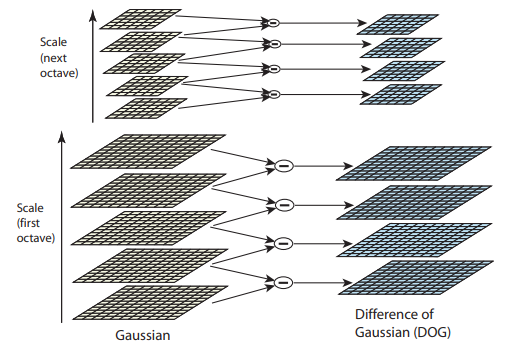
\includegraphics[width=0.6\linewidth]{figures/c3/Hình 1 paper sift.png}
    \caption{Tạo không gian Hiệu số Gauss từ các tầng ảnh khác nhau \cite[Fig.~1]{Lowe04Distinctive}.}
    \label{fig:dog}
\end{figure}

Hàm $L(x, y, \sigma)$ biểu diễn hình ảnh ở mức độ làm mờ với tham số tỷ lệ $\sigma$. Tháp Gaussian được xây dựng bằng cách tăng dần $\sigma$ trong mỗi tầng của tháp và giảm kích thước hình ảnh ở các tầng cao hơn để giảm chi phí tính toán. Để phát hiện các điểm đặc trưng bất biến tỷ lệ, SIFT sử dụng không gian Hiệu số Gauss (DoG) - mô tả tại Hình \ref{fig:dog}, được tạo nên bằng cách tính bằng hiệu của hai hình ảnh làm mờ ở các mức độ $\sigma$ khác nhau trong cùng 1 tầng:

\begin{equation}
D(x, y, \sigma) = L(x, y, k\sigma) - L(x, y, \sigma),
\end{equation}
với $k$ là hằng số nhân tỷ lệ (thường $k = 2^{1/s}$, $s$ là số mức trong một tầng). Hàm $D(x, y, \sigma)$ gần đúng với Laplacian của Gaussian, giúp phát hiện các vùng có sự thay đổi cường độ đáng kể, tương ứng với các đặc trưng tiềm năng.

\begin{figure}[H]
    \centering
    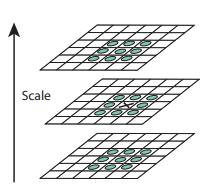
\includegraphics[width=0.4\linewidth]{figures/c3/so_sanh_x_vs_26p_Hinh_2_sift.png}
    \caption{Mô tả vùng lân cận của điểm X được sử dụng để tìm cực trị\cite[Fig.~2]{Lowe04Distinctive}.}
    \label{fig:lan_can_x}
\end{figure}

Các điểm cực trị trong không gian DoG được xác định bằng cách so sánh mỗi điểm trong hình ảnh DoG với các điểm lân cận của nó trong không gian 3D được mô tả trong Hình \ref{fig:lan_can_x} . Giả sử bạn đang xét điểm $(x, y, \sigma_i)$ trong hình ảnh DoG tại mức làm mờ $\sigma_i$. Vùng lân cận 3D có thể được mô tả như một khối 3x3x3 (3 điểm ảnh theo $x$, 3 điểm ảnh theo $y$, 3 mức tỷ lệ mờ lần lượt là $\sigma_{i-1}$, $\sigma$, $\sigma_{i11}$), với điểm đang xét nằm ở trung tâm (Các hình ảnh DoG này nằm trên cùng 1 tầng kích thước). Tổng số điểm trong khối này là $3 \times 3 \times 3 = 27$, do đó, mỗi điểm sẽ so sánh giá trị với 26 điểm lân cận còn lại.
Một điểm được coi là cực trị nếu nó có giá trị lớn nhất hoặc nhỏ nhất trong vùng lân cận đó. Những điểm này là ứng viên cho các điểm đặc trưng. 

\subsection{Tinh chỉnh vị trí điểm đặc trưng}

Sau khi xác định các điểm cực trị, SIFT tinh chỉnh vị trí và loại bỏ các điểm không ổn định. Vị trí chính xác của điểm đặc trưng được xác định bằng cách sử dụng xấp xỉ Taylor bậc hai của hàm $D(x, y, \sigma)$ quanh điểm cực trị:

\begin{equation}
D(\mathbf{x}) = D + \frac{\partial D}{\partial \mathbf{x}}^T \mathbf{x} + \frac{1}{2} \mathbf{x}^T \frac{\partial^2 D}{\partial \mathbf{x}^2} \mathbf{x},
\end{equation}
trong đó $\mathbf{x} = (x, y, \sigma)^T$ là vector vị trí và tỷ lệ. Điểm cực trị được tìm bằng cách lấy đạo hàm và đặt bằng 0:

\begin{equation}
\hat{\mathbf{x}} = -\left( \frac{\partial^2 D}{\partial \mathbf{x}^2} \right)^{-1} \frac{\partial D}{\partial \mathbf{x}}.
\end{equation}

Nếu giá trị $|\hat{\mathbf{x}}|$ quá lớn (vượt ngưỡng, ví dụ 0.5 theo đơn vị pixel), điểm cực trị được coi là không ổn định và bị loại bỏ. Ngoài ra, các điểm có độ tương phản thấp (giá trị $|D(\hat{\mathbf{x}})|$ nhỏ) hoặc nằm trên cạnh cũng bị loại bỏ để đảm bảo tính ổn định.

\subsection{Gán hướng cho điểm đặc trưng}

Để đảm bảo tính bất biến xoay, mỗi điểm đặc trưng được gán một hướng chính dựa trên gradient của hình ảnh xung quanh. Gradient tại điểm $(x, y)$ trong hình ảnh $L(x, y, \sigma)$ được tính như sau:

\begin{equation}
m(x, y) = \sqrt{\left( L(x+1, y) - L(x-1, y) \right)^2 + \left( L(x, y+1) - L(x, y-1) \right)^2},
\end{equation}

\begin{equation}
\theta(x, y) = \tan^{-1} \left( \frac{L(x, y+1) - L(x, y-1)}{L(x+1, y) - L(x-1, y)} \right).
\end{equation}

Trong đó, $m(x, y)$ là độ lớn gradient và $\theta(x, y)$ là hướng gradient. Các hướng gradient trong một vùng xung quanh điểm đặc trưng được tổng hợp thành một histogram hướng. Đỉnh cao nhất trong histogram được chọn làm hướng chính, và các đỉnh phụ (nếu vượt 80\% giá trị đỉnh chính \cite{Lowe04Distinctive}) cũng có thể được sử dụng để tạo thêm điểm đặc trưng, tăng tính mạnh mẽ.

\subsection{Mô tả đặc trưng SIFT}

Cuối cùng, SIFT tạo ra một vector mô tả đặc trưng cho mỗi điểm đặc trưng, đảm bảo tính bất biến với thay đổi tỷ lệ, xoay và ánh sáng. Một vùng xung quanh điểm đặc trưng (kích thước tỷ lệ với $\sigma$) được chia thành lưới 4x4 ô. Trong mỗi ô, gradient được tổng hợp thành histogram hướng với 8 khoảng giá trị (chia đều 360 độ thành 8 khoảng giá trị). Từ đó, tổng hợp ra vector mô tả cuối cùng là một vector 128 chiều (4x4x8), được chuẩn hóa để loại bỏ ảnh hưởng của thay đổi ánh sáng.

Quá trình chuẩn hóa bao gồm việc chia vector cho độ lớn Euclidean của nó:

\begin{equation}
\mathbf{d} = \frac{\mathbf{d}}{\|\mathbf{d}\|_2},
\end{equation}
trong đó $\mathbf{d}$ là vector mô tả. Để giảm ảnh hưởng của các giá trị gradient lớn, các phần tử trong vector được giới hạn (thường ở mức 0.2) và vector được chuẩn hóa lại.

\subsection{Ý nghĩa của SIFT}

SIFT nổi bật nhờ khả năng tạo ra các đặc trưng cục bộ mạnh mẽ, bất biến với các biến đổi hình học. Những tính chất này làm cho SIFT trở thành một công cụ quan trọng trong các ứng dụng SfM, nơi cần khớp các điểm đặc trưng giữa các hình ảnh có góc nhìn và điều kiện khác nhau.
